\documentclass{article}

% Lecture notes theme files
\usepackage{Layout/lecturenotes}

\usepackage{natbib}
\bibliographystyle{abbrvnat}
\setcitestyle{authoryear,open={(},close={)}} %Citation-related commands

\usepackage{import}
\import{Layout/}{definitions.tex}

%%%% Title
\title{Decomposition methods for stochastic programming and \linebreak robust optimisation}
\author{Fabricio Oliveira}

\begin{document}

%%%% Setting cover page
\begin{titlepage}
\singlespacing
\thispagestyle{empty}

\maketitle

\begin{abstract} In this lecture series, we will introduce the basics of some of the main variants of decomposition methods that can be employed to tackle large-scale stochastic programming problems. We will focus on two-stage stochastic programming (2SSP) models for simplicity, pointing out how they can be generalised for multi-stage settings. 

We focus on four methods, namely Benders decomposition (or the L-shaped method), column-and-constraint generation, Lagrangian decomposition and progressive hedging. We will focus on describing how they work and illustrate some of their main differences while keeping the exposition not overly technical.
 
\end{abstract}

\tableofcontents
\end{titlepage}

\onehalfspacing

%%%% Content starts from here

\part{Stochastic programming}

\section{Introduction: stochastic programming problems}

We start by considering the type of mathematical programming problems we are interested in solving. Let $x \in \reals^n \times \braces{0,1}^p$, to which we will refer to as \emph{first-stage} variables. Also, assume that a set of \emph{scenarios} are defined and represented by $s \in S$.

We can then define \emph{second-stage} variables $y_s \in \reals^m \times \braces{0,1}^q$, $\forall s \in S$, which represent decisions made after the realisation of a given scenario $s \in S$ is observed.

In its simplest form, a two-stage stochastic programming (2SSP) problem can be stated as follows
%
\begin{align*}
	\mini & c^\top x + \sum_s p_s q_s^\top y_s \\	
	\st   & Ax = b \\
		  & T_s x + W_s y = h_s, \ \forall s \in S \\
		  & x \in X, \\
		  & y_s \in Y_s, \forall s \in S.	
\end{align*}

Parameters $c$, $b$, $p_s$ and $q_s$ are all of adequate size. Assume that $A$ has $c_1$ rows, while $T_s$ and $W_s$ have $c_2$ rows. The sets $X$ and $Y_s$, $\forall s \in S$, define bounds and nonnegativity conditions of the continuous variables.
 
 Notice that this is a rather general formulation. Furthermore, it can be adapted to encompass more stages, say $T$ stages, creating a ``nesting'' effect, where, at each stage $t$, the variables associated with $t-1$ act as first-stage variables. For example, a $T=3$-stage problem can be formulated as follows.
%
\begin{align}
	\mini & c^\top x + \sum_{s^1 \in S^1} p_{s^1} \left[ (q^1_{s^1})^\top y^1_{s^1}  + \sum_{s^2 \in S^2} p^2_{s^2} (q^2_{s^2})^\top y^2_{s^2}\right] \\	
	\st   & Ax = b \\
		  & T^1_{s^1} x + W^1_{s^1}y^1_{s^1} = h^1_{s^1}, \ \forall s^1 \in S^1 \\
		  & T^2_{s^2} x + W^2_{s^2}y^2_{s^2} = h^2_{s^2}, \ \forall s^2 \in S^2 \\
		  & x \in X, \\
		  & y^1_{s^1} \in Y^1_{s^1}, \forall s^1 \in S^1 \\	
		  & y^2_{s^2} \in Y^2_{s^2}, \forall s^2 \in S^2. \\
\end{align}


Graphically, the problem would have a structure as presented in figure \ref{fig:problem_structure}.

\begin{figure}[h]
	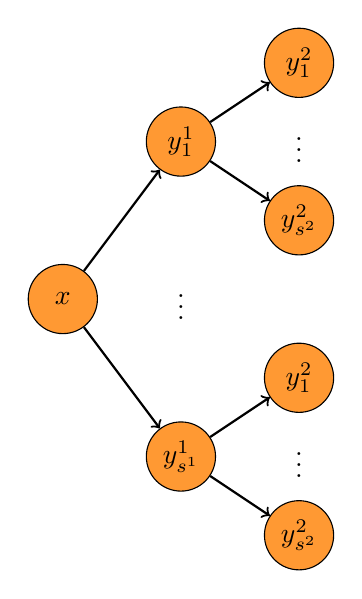
\begin{tikzpicture}
	    [chance/.style={circle, fill=orange!80, draw, minimum size=2.5em, inner sep=2pt}, scale=1]
	    % \draw[step=1cm,gray,very thin] (0,0) grid (5,5);
	    \node[chance]   (B1) at (0,0)    {$x$};
	    \node[chance]   (C1) at (1.5,2)  {$y_1^1$};
	    \node[chance]   (C2) at (1.5,-2) {$y^1_{s^1}$};
	    \node[chance]   (D1) at (3,3)    {$y^2_1$};
	    \node[chance]   (D2) at (3,1)    {$y^2_{s^2}$};
	    \node[chance]   (D3) at (3,-1)   {$y^2_1$};
	    \node[chance]   (D4) at (3,-3)   {$y^2_{s^2}$};
	    \node (dots1) at (1.5, 0) {$\vdots$};
	    \node (dots2) at (3, 2) {$\vdots$};
	    \node (dots3) at (3, -2) {$\vdots$};    
	    \draw[->, thick] (C1) -- (D1);
	    \draw[->, thick] (C1) -- (D2);
	    \draw[->, thick] (C2) -- (D3);
	    \draw[->, thick] (C2) -- (D4);
	    \draw[->,  thick] (B1) -- (C1);
	    \draw[->,  thick] (B1) -- (C2);
	\end{tikzpicture} 
	\caption{Representation of the problem structure of a 3-stage stochastic problems. The circles represent stages, at which a decision is made and the branches represent scenarios.} \label{fig:problem_structure}
\end{figure}

In what follows, we will concentrate on 2SSP models for simplicity, but most of the methods we will see have an equivalent form for multi-stage settings.

\section{Decomposition: motivation}

One critical aspect of stochastic programming models is that having multiple scenarios and stages rapidly increases the scale of the model. This typically poses issues related to their practical applicability due to steep computational requirements.

Therefore, one often must rely on methods that allow for breaking these problems into smaller and more manageable parts that can be recombined into a solution to the original problem. Moreover, this can often be done in a way that reaps benefits from parallelisation, leading to even further solution time speed-ups. 

Two types of separation can be performed on a given mathematical programming model, and they differ according to the \emph{complicating structure} of the problem. The complicating structure is simply the set of \emph{variables} or \emph{constraints} that prevent the problem from being solved as separated parts.

Let us consider our 2SSP in the following form:

\begin{tabular}{rccccc}
	$\mini$ & $c^\top x$ & + $p_1 q_1^\top y_1$ & $\dots$ & + $p_{|S|} q_{|S|}^\top y_{|S|}$ &     \\
	$\st$   & $Ax$       &                      &         &   	                           & = $b$ \\
	        & $T_1x$     & + $W_1y_1$           &         &   	                           & = $h_1$ \\
	        &		    &	                      & $\ddots$&                                  &    \\   
	        & $T_{|S|}x$ &                      &         & + $W_{|S|}y_{|S|}$              & = $h_{|S|}$. \\
\end{tabular}

Notice that if the value of $x$ is set, the problem can be solved as a collection of $|S|$ problems that are \emph{independent} of each other. This is why we say that $x$ is a \emph{complicating variable}.

The other type consists of \emph{complicating constraints}. To see that, let us first restate our 2SSP as 
%
\begin{align*}
	\mini & \sum_s P_s\left(c^\top x_s + q_s^\top y_s\right) \\	
	\st   & Ax_s = b, \forall s \in S \\
		  & T_s x + W_s y = h_s, \ \forall s \in S \\
		  & x_s \in X, \ \forall s \in S \\
		  & y_s \in Y_s, \forall s \in S \\
		  & x_1 = \dots = x_{|S|}.	
\end{align*}

The constraint $x_1 = \dots = x_{|S|}$ is known as the \emph{nonanticipativity conditions} (NAC), since it enforces that the solution $x$ cannot anticipate which scenario may unveil. Now, notice that the structure of the 2SSP model is slightly different.

\begin{tabular}{rccccc}
	$\mini$ & $p_1(c_1^\top x_1 + q_q ^\top y_1)$ & $p_2(c_2^\top x_2 + q_2 ^\top y_2)$ & $\dots$ & $p_{|S|}(c_{|S|}^\top x_{|S|} + q_{|S|} ^\top y_{|S|})$ & \\
	$\st$ & $Ax_1$ & & & & $=b$ \\
	& $Tx_1 + W_1y_1$& & & & $=h_1$ \\  
	& & $Ax_2$ & & & $=b$ \\
	& & $Tx_2 + W_2y_2$ & & & $=h_2$ \\
	& & & $\ddots$ & & \\   
	& & & & $Tx_{|S|} + W_{|S|}y_{|S|}$ & $=h_{|S|}$ \\
	& $x_1$ & & & & $= x_{|S|}$ \\
	& & $x_2$ & & & $= x_{|S|}$
\end{tabular}

Notice that what prevents separability now are the constraints that enforce the NAC. In this case, we say that they are \emph{complicating constraints}.

In these lectures, we will discuss four methods, namely
\begin{itemize}
	\item \textbf{Benders decomposition and constraint-and-column generation}: for formulations with complicating variables.
	\item \textbf{Lagrangian decomposition and progressive hedging}: for formulations with complicating constraints.	
\end{itemize}



\pagebreak
\part{Benders decomposition}

\section{Benders decomposition for 2SSP}

Benders decomposition is a delayed constraint generation approach. To see how it works, let us first split our problem as 
%
\begin{align*}
	\mini & c^\top x + \mathcal{Q}(x) \\
	\st   & Ax = b \\
		  & x \in X			
\end{align*}

where $\mathcal{Q}(x)$ is defined as
%
\begin{align*}
	\mathcal{Q}(x) = \mini & \sum_s p_s q_s^\top y_s \\	
	\st & W_s y_s = h_s - T_s x, \ \forall s \in S.
\end{align*}

Notice that $\mathcal{Q}(x)$ is separable scenario-wise, i.e., can be solved separately for each $s \in S$. Now, let us consider the dual formulation of $Q(x)$.
%
\begin{align*}
	\mathcal{Q}(x) = \maxi & \sum_s \pi_s ^\top (h_s - T_s x) \\	
	\st & W_s \pi_s \leq p_s q_s, \ \forall s \in S.
\end{align*}

Since we are using linear programming duality, we must require that all second-stage variables $y_s$, $\forall s \in S$ are continuous (i.e., $q = 0$). This is an assumption that can be relaxed using an alternative variant of the method \citep{LAPORTE1993}, but we will leave this discussion out for now. 

Since the dual of $Q(x)$ (and $Q(x)$) is a linear programming problem, we know that it has an equivalent representation based on a finite number of extreme points (vertices) and extreme rays. For simplicity, let us assume that we have \emph{relatively complete recourse}, meaning that $Q(x)$ is feasible for any value of $x$ satisfying $Ax = b$ and $x \in X$. This allows us to preclude the treatment of extreme rays since the dual form of $Q(x)$ cannot be unbounded (which is the case for an infeasible $Q(x)$).

If we knew all extreme points $\pi^k = (\pi_s^k)_{s \in S}$, $k = 1, \dots, K$ of the feasible region of the dual of $Q(x)$, we could rewrite our original 2SSP as
%
\begin{align*}
	\mini & c^\top x + \theta \\
	\st   & \theta \geq \sum_s (\pi_s^k)^\top (h_s - T_s x),\ k = 1, \dots, K \\
	&Ax = b \\
	& x \in X.	
\end{align*}

Notice that this would allow us to represent the subproblem $\mathcal{Q}(x)$ as a piecewise linear function of $x$. Naturally, assuming that all extreme points $\braces{\pi^k}_{k=1,\dots,K}$ are available is not a practical assumption. However, we can iteratively generate them ``on the fly'', one at a time, and proceed to incrementally adding cuts (or constraints) of the form
%
\begin{equation*}
	\theta \geq \sum_{s \in S}(\pi_s^k)^\top(h_s - T_s x).	
\end{equation*}

Notice that this is equivalent to iteratively reconstructing the whole set of $K$ vertices, in which the choice of $x$ is guided by a current \emph{approximation} of the piecewise linear function representing $\mathcal{Q}(x)$.

The method can be summarised as follows:

\begin{enumerate}
	\item[\bf Step 1:] Initialisation. Set $LB = -\infty$, $UB = \infty$, $k=0$. 
	\item[\bf Step 2:] Solve the \emph{main problem} $M^k$
	\begin{align*}
		M^k: \mini & c^\top x + \theta \\
		     \st & \theta \geq \sum_s (\pi_s^k)^\top (h_s - T_s x), \ k = 1, \dots K, \\
		     & Ax = b \\
		     & x \in X. 	
	\end{align*} 
	%
	Let $\underline{z}^k = c^\top x^k + \theta^k$, where $(x^k, \theta^k)$ are the optimal solutions of $M^k$. Make $LB = \underline{z}^k$.
	\item[\bf Step 3:] Solve the subproblem $SP(x^k)$
	\begin{align*}
		SP(x^k): \maxi & \sum_s \pi_s ^\top (h_s - T_s x^k) \\
		     \st & W_s^\top \pi_s  \leq p_s q_s, \ \forall s \in S.
	\end{align*}  
	%
	Let $\overline{z}^k = \sum_s (\pi_s^k)^\top (h_s - Tsx^k)$, where $(\pi_s^k)_{s \in S}$ is the optimal solution of $SP(x^k)$. Make $UB = \min\braces{UB, \overline{z}^k}$. If $UB - LB < \epsilon$, return $x^k$ as optimal solution. 
	\item[\bf Step 4:] Make $k = k+1$. Generate constraint 
	\begin{equation*}
		\theta \geq \sum_s (\pi_s^k)^\top (h_s - T_s x)
	\end{equation*}
	%
	and add it to $MP^k$. Return to Step 2.
\end{enumerate}

Some final remarks:
\begin{enumerate}
	\item It may be that the subproblem is infeasible, in case the assumption concerning the relative completeness of the recourse does not hold. In this case, instead of an optimality cut, a feasibility cut of the form
		\begin{equation*}
			\sum_s (\pi_s^k)^\top (h_s - T_s x) \leq 0,
		\end{equation*}
		%
 		must be generated since, in this case, $\pi_s^k$, $\forall s \in S$, represents an extreme ray (or unbounded direction).
	\item It is likely that the main problem is unbounded in the first few iterations. Ideally, one should impose trust regions or generate a couple of feasible solutions $x$ to prepolulate it with cuts. 
	\item \cite{BIRGE1988} proposed a multi-cut version, in which the main problem is modified as
	\begin{align*}
		M^k_{\text{multi}}: \mini & c^\top x + \sum_s \theta_s \\
		     \st & \theta_s \geq (\pi_s^k)^\top (h_s - T_s x), \  \forall s \in S, k = 1, \dots K, \\
		     & Ax = b \\
		     & x \in X. 	
	\end{align*}
	%
	This exploits the separability of the subproblem and can be beneficial for convergence at the expense of a faster increase in the main problem size as the iterations progress, as more constraints are generated per iteration (one per scenario $s \in S$). 
	\item There are in the literature ideas known as \emph{acceleration techniques}, which are modifications in the Benders decomposition aimed at minimising the number of iterations required for convergence. \citet{OLIVEIRA2014} and \citet{PLACIDO2019} are some of my own work discussing acceleration ideas. The literature review from \citet{RAHMANIANI2017} has pointers to several acceleration ideas while also discussing other key aspects related to the method.
	\item One important related method (that we will not cover in these lectures) is the stochastic dual dynamic programming (SDDP) originally proposed by \citet{PEREIRA1999}. SDDP can be understood as having the L-shaped method applied to a multi-stage stochastic programming problem, in which each stage is solved sequentially, based on a current approximation of the expected value of the future stages and on via sampling of the uncertainty.  
\end{enumerate}


\pagebreak
\part{Column and constraint generation}

\section{Introduction}

Now we turn our focus to a specific type of optimisation under uncertainty in which we consider risk-averseness and robustness. A two-stage (or adaptable) robust optimisation model has the following form.
%
\begin{align*}
	\min_x \ & c^\top x + \max_{u \in \mathcal{U}} \min_{y} q^\top y \\
	\st   & Ax = b \\
	& x \in X \\
	& Tx = h - Wy - Mu \\
	& y \in Y.
\end{align*}
%
As before, we have that $x \in \reals^{n} \times \braces{0,1}^p$, $y \in \reals^m \times \braces{0,1}^q$. All matrices and vectors are assumed of appropriate sizes. The set $\mathcal{U}$ is known as the \emph{uncertainty set}, which can be, e.g., a discrete set of scenarios or a polyhedral set.

Essentially, this tri-level problem is searching for a first-stage solution that minimises the response (second-stage) cost associated with the most adverse realisation of the uncertain variable $u$ within the uncertainty set $\mathcal{U}$.


\section{A min-max approach}

First, let us assume that $\mathcal{U}$ is finite and discrete. Then, we can say that each element in $\mathcal{U} = \braces{u_1, \dots, u_{|S|}}$ acts as a ``scenario'', with associated set of (second-stage) variables $y_s$, $\forall s \in S = \braces{1, \dots, |S|}$.

This allows us to reformulate our problem into a deterministic equivalent form as follows.
%
\begin{align*}
	\mini & c^\top x + \theta \\
	\st & Ax = b \\
	& x \in X \\
	& \theta \geq q^\top y_s, \ \forall s \in S \\
	& Tx = h - Wy_s - Mu_s \ \forall s \in S \\
	& y_s \in Y, \forall s \in S.
\end{align*}
%
Notice that this might still be a large-scale problem. However, we can see that if we have a method to optimally choose \emph{non-trivial (or critical) scenarios}, we can start from a subset of scenarios $S = \braces{1, \dots, r}$ and gradually augment it until convergence is observed. 


\section{Column-and-constraint generation}

The column-and-constraint generation (CCG) method \citep{ZENG2013} is based on the idea of iteratively generating critical scenarios. In particular, it is designed to iteratively expand the uncertainty set $\mathcal{U}$ by identifying and including critical scenarios and generating respective recourse decisions as the algorithm progresses.

First, let us restate our problem as 
%
\begin{align*}
	\mini & c^\top x + \mathcal{Q}(x) \\
	& Ax = b \\
	& x \in X,
\end{align*}
%
where 
\begin{equation*}
	\mathcal{Q}(x)	 = \braces{\max_{u \in \mathcal{U}} \min_y q^\top y : Tx = h - Wy - Mu, y \in Y}.
\end{equation*}
%
Assume that we have an \emph{oracle} that can solve $Q(x)$ for any given $x$ and returns an optimal solution $(y^*, u^*)$ if it exists. The CCG method can be summarised as follows.

\begin{enumerate}
	\item[\bf Step 1:] Initialisation. $LB = -\infty$, $UB = \infty$, $k = 0$.
	\item[\bf Step 2:] Solve the main problem $M^k$
	\begin{align*}
		M^k: \mini_{x,y,\theta} & c^\top x + \theta \\
		& Ax = b \\
		& x \in X \\
		& \theta \geq q^\top y_s, s = 1, \dots, k \\
		& Tx = h - Wy_s - M\overline{u}_s, s = 1, \dots, k \\
		& y_s \in Y, s = 1, \dots, k.
	\end{align*}
	%
	Let $\underline{z}^k = c^\top x^k + \theta^k$, where $(x^k, \theta^k, (y_s^k)_{s=1}^k)$ form the optimal solution of $M^k$. Make $LB = \underline{z}^k$.
	\item[\bf Step 3:] call the oracle that solves $\mathcal{Q}(x^k)$. Let $(\overline{u}^{k+1}, y^{k+1})$ be the optimal solution returned by the oracle, if it exists. Let $\overline{z}^{k} = c^\top x^k + \mathcal{Q}(x^k)$. Make  $UB = \min\braces{UB, \overline{z}^{k}}$. If $UB = LB < \epsilon$, return $x^k$ as the optimal solution.
	\item [\bf Step 4:] if $\mathcal{Q}(x^k) < \infty$ (i.e., is feasible), create variables $y_{k+1}$ and add them to the main problem, together with the constraints
	\begin{align*}
		& \theta \geq q^\top y_{k+1} \\
		& Tx = h - Wy_{k+1} - M\overline{u}^{k+1}
	\end{align*}
  	to form $M^{k+1}$. Make $k = k+1$ and return to Step 2. If $\mathcal{Q}(x^k)$ is not feasible, then only the second constraint needs to be created.
\end{enumerate}


\section{Solving the inner problem: the oracle for $\mathcal{Q}(x)$}

The final part missing for having a practical algorithm is the definition of the oracle that is called to solve $\mathcal{Q}(x)$. Recall that $\mathcal{Q}(x)$ is of the form:
%
\begin{align*}
	\mathcal{Q}(x)	 = &\max_u q^\top y    \\
	   \st &u \in \mathcal{U}  \\ 	 
		   &y \in \argmin_y q^\top y \\
	       &\qquad \quad \st Tx = h - Wy - Mu \\
		   &\qquad \qquad \quad \ y \in Y.	
\end{align*}

Essentially, $\mathcal{Q}(x)$ is a \emph{bilevel problem} that must (in general) be reformulated into a tractable equivalent single-level problem in order to be appropriately solved. This can be achieved by employing a variety of different approaches, in which most, if not all, rely on the convexity of the lowermost problem. 

For example, for a fixed $u \in \mathcal{U}$, assuming that $y \in \reals^m$ and disregarding the set $Y$\footnote{the set $Y$ can be incorporated into the set of constraints $Tx = h - Wy - Mu$ by making $T$ and $M$ null matrices.}  we can use strong duality to reformulate the inner problem, obtaining
%
\begin{align*}
	\mathcal{Q}(x) = &\max_{u,\pi} (h - Tx - Mu)^\top \pi \\
	   \st & \pi^\top W = q^\top \\
	   	   &u \in \mathcal{U}	 
\end{align*}
%
which is tractable, if 
\begin{enumerate}
	\item $u$ is integer or has a discrete domain, since $u^\top \pi$ can be reformulated exactly;
	\item if $M$ is positive semi-definite, since we would be maximising a concave quadratic function;
	\item if applying spatial branch-and-bound (e.g., Gurobi's spatial branch-and-bound method) is feasible from a computational standpoint.	
\end{enumerate}

Some final remarks: 

\begin{enumerate}
	\item The CCG method can be seen as a primal equivalent of the Benders decomposition. In fact, one can use the same idea of generating primal variables and constraints to the main problem in the context of the L-Shaped method. \citet{GAMBOA2021} shows a comparison between variants of the L-Shaped method and CCG for the 2SSP problem.
	\item Notice that convergence relies on a finiteness argument on the uncertainty set. For convergence to be guaranteed, we must require that, for example, $\mathcal{U}$ is a set of discrete elements or a polyhedral set (thus with a finite number of extreme points and rays).
\end{enumerate}


\pagebreak
\part{Lagrangian (dual) decomposition}

\section{Introduction}

We now consider an alternative framework for decomposition, which is based on more general Lagrangian duality. In contrast with Benders decomposition, Lagrangian decomposition does not require convexity of the subproblem for converging, but only of its \emph{linear relaxation}. This is why these methods are often seen as better suited for stochastic mixed-integer programming problems. 

\textbf{Remark:} the above is not entirely true. Since the 90's (see Laporte and Louveaux 1993), there have been developments that allow for the employment of Benders (or the L-Shaped method) to problems with integer variables in the second stage.

One truly remarkable feature of Lagrangian decomposition approaches is their amenability to parallelisation. Before we discuss this aspect in more details, let us first describe the method.

\section{A reformulations strategy}

As we discussed earlier, Lagrangian decomposition is suited for obtaining separability in the presence of \emph{complicating constraints}. Recall the structure of our 2SSP.
%
\begin{align*}
	\mini & c^\top x + \sum_s p_s q_s^\top y_s \\
	\st   & Ax = b \\
	& T_s x + W_s y_s = h_s, \ \forall s \in S \\
	& x \in X \\
	& y_s \in Y_s \ \forall s \in S.	
\end{align*}

As we discussed earlier, the complicating structure is associated with the first-stage variables $x$. Thus, in order to expose the complicating structure by means of constraints, we have to perform the following reformulation.
%
\begin{align*}
	\mini &\sum_s p_s(c^\top x_s + q_s^\top y_s) \\	
	\st & Ax_s = b, \ \forall s \in S \\
	& Tsx_s + W_sy_s = h_s, \ \forall s \in S \\
	& x_s \in X, \ \forall s \in S \\
	& y_s \in Y_s, \ \forall s \in S \\
	& x_1 = x_2 = \dots = x_{|S|}. 
\end{align*}
%
In effect, this reformulation is based on generating copies of the first-stage variable $x_s$, one for each scenario $s \in S$, that are then connected via the constraint $x_1 = x_2 = \dots = x_{|S|}$. This constraint is known as the \emph{nonanticipativity conditions} (NAC), meaning that it prevents the first-stage decision $x$ from anticipating a specific scenario.

Specifically, nonanticipativity constraints can have several forms. Some examples:
%
\begin{enumerate}
	\item symmetric: $x_s = x_{s+1}$, for $s \in \braces{1,\dots,|S|-1}$.
	\item asymmetric: $x_{\overline{s}} = x_{s}$, for $s \in S \setminus {\overline{s}}$.
\end{enumerate}
 %
 As one might suspect, since the representation of the NACs is not unique, different options might have different impacts on the observed performance of the algorithm.
 

\section{Using Lagrangian relaxation to obtain a decomposition}
 
One can notice that, once the nonanticipativity conditions are removed, the problem can be decomposed scenario-wise. In what follows, let us assume that we adopt the asymmetric representation of the NAC. Then, employing Lagrangian relaxation to the NAC yield the \emph{Lagrangian function}
%
\begin{align*}
	L(\lambda) = \mini & \sum_s p_s (c^\top x_s + q_s ^\top y_s) + \sum_s \lambda_s g_s \\
 	\st & Ax_s = b, \ \forall s \in S \\
 	& T_sx_s + W_sy_s = h_s, \ \forall s �n S \\
 	& x_s \in X, \ \forall s \in S \\
 	& y_s \in Y_s, \ \forall s \in S, 
\end{align*}
%
where $g_s = x_{\overline{s}} - x_s$, $\forall s \in S \setminus \{\overline{s}\}$. Notice that the Lagrangian function is completely separable scenario-wise. To see that, we can redefine it as
%
\begin{equation*}
	L(\lambda) = \sum_s L_s(\lambda),	
\end{equation*}
%
where $L_s(\lambda)$ is given by
%
\begin{align*}
	L(\lambda) = \mini & \sum_s p_s (c^\top x_s + q_s ^\top y_s) + \sum_s \lambda_s f_s(\lambda)x_s \\
 	\st & Ax_s = b \\
 	& T_sx_s + W_sy_s = h_s \\
 	& x_s \in X \\ 
 	& y_s \in Y_s  
\end{align*}
%
with $f_s(\lambda)$ simply being
\begin{equation*}
	f_s(\lambda) = 
	\begin{cases}
		\sum_{s \in S \setminus \{\overline{s}\}} \lambda_s, \text{ if } s = \overline{s} \\
		-\lambda_s, \text{ otherwise.}	
	\end{cases}
\end{equation*}

Notice that \emph{evaluating} the Lagrangian function requires solving the 2SSP, given an argument $\lambda = (\lambda_s)_{s \in S}$. These multipliers $\lambda$ are the so-called \emph{Lagrangian multipliers}.

The theoretical framework under which this idea is developed is known as \emph{Lagrangian duality}, to which linear programming duality is a special case. The key result of our interest in this context is known as \emph{weak duality}, which states the following. Let $z^*$ be the optimal objective value of the 2SSP. Then, we have that, for any $\lambda$,
%
\begin{equation*}
	L(\lambda) \leq z^*.
\end{equation*}

Lagrangian duality-based methods typically employ optimisation to find the best possible bound provided by $L(\lambda)$, which can be obtained solving the \emph{Lagrangian dual problem}
%
\begin{equation*}
	\max_\lambda L(\lambda).
\end{equation*}
%
Under convexity and a constraint qualification condition\footnote{Conditions that, once satisfied by a constraint set, allow for creating a link between Karush-Kuhn-Tucker conditions and optimality of a feasible point.}, it can be shown that
%
\begin{equation*}
	\max_\lambda L(\lambda) = z^*.
\end{equation*}

The strongest selling point of Lagrangian decomposition methods is that, for each $\lambda$, evaluating the Lagrangian dual function can be done in parallel, with very little structure to be shared. This means that there is no central main problem that increases as iterations progress and that the largest problem solved is as large as a single scenario problem.

\section{Solving the Lagrangian dual}

The Lagrangian dual problem is, in essence, a bi-level problem and, thus, require specific solution techniques. For linear 2SSP models, and more generally general for any other problem, the Lagrangian dual problem is a piecewise linear concave function. This means that a nonsmooth optimisation problem must be employed to solve it. The most common methods are:

\begin{itemize}
	\item subgradient method;
	\item cutting plane method;
	\item bundle methods.
\end{itemize}

We will discuss in more detail the subgradient method.


\subsection{The subgradient method}

The subgradient method is based on the idea of successively taking ascending subgradient steps in the space of the Lagrangian dual variables. 

The subgradient is a generalisation of the gradient for non-differentiable functions. In our particular case, $g_s$, $\forall s \in S$ is a subgradient for $L_s(\lambda)$. As we would like to maximise $L(\lambda)$, we can take steps of the form
%
\begin{equation*}
	\lambda_s^{k+1} = \lambda_s^{k} + \mu^k g^k_s, \ \forall s \in S,
\end{equation*}
%
where $k$ is an iteration counter and $\mu^k_s$ is a step size. There are multiple alternative ways to define the step-size term, many of them drawing from techniques used in variants of the gradient/ steepest descent method. One common update rule is that known as the \emph{Polyak} rule, which is given by
%
\begin{equation*}
	\mu^k = \alpha_k \frac{\overline{z} - L(\lambda^k)}{||(g_s)_{s \in S}||^2},	
\end{equation*}
%
where $\overline{z}$ is an upper bound on the optimal solution of the 2SSP $z^*$, $L(\lambda^k)$ is the value of the Lagrangian dual function, evaluated at iteration $k$. 


\section{Dual decomposition (DD) method}

The DD method can be summarised as follows

\begin{enumerate}
	\item[\bf Step 1:] Initialisation. $LB = \infty$, $k=0$, $\lambda^k = \overline{\lambda}$.
	\item[\bf Step 2:] Evaluate the Lagrangian dual function 
	%
	\begin{align*}
		L(\lambda^k) = \mini & \sum_s p_s (c^\top x_s + q_s ^\top y_s) + \sum_s \lambda^k_s g_s \\
			\st & Ax_s = b, \ \forall s \in S \\
			& T_sx_s + W_sy_s = h_s, \ \forall s �n S \\
			& x_s \in X, \ \forall s \in S \\
			& y_s \in Y_s, \ \forall s \in S, 
	\end{align*}
	%
	obtaining $(x_s^k, y_s^k)_"{s \in S}$. $LB^{k+1} = \max\braces{L(\lambda^k), LB^k}$.
	\item[\bf Step 3:] If $||(g_s)_s \in S|| < \epsilon$, return $(x_s^k, y_s^k)$ and $LB^{k+1}$. Otherwise, $k=k+1$, update $\lambda^k$ using the chosen method and return to Step 2.	 		
\end{enumerate}

One point to remark is that, if the evaluation of the Lagrangian dual function requires one to solve MIPs, strong duality may not hold. This means that solving the Lagrangian dual problem is at best a \emph{bounding techinque} that can be combined with branching strategies to find an optimal solution. The combination of a branching strategy specialised for NAC conditions and bounding using Lagrangian decomposition is known as dual decomposition (Car�e and Schultz, 1998) 


\pagebreak
\part{Progressive hedging}

Progressive hedging (PH) is a method also based on Lagrangian decomposition. However, it relies on additional features to allow for complete separation while recovering the differentiability of the Lagrangian dual function.

PH can be seen as a special case of a more general algorithm known as the alternating direction method of multipliers (ADMM) which has as most important feature allowing for the solution of problem in a decoupled (or decomposed) form.


\section{A formulation for PH}

PH requires a specific reformulation of our 2SSP. Again, let us consider the problem
%
\begin{align*}
	\mini &c^\top x + \sum_s p_s q_s ^\top y_s \\ 
	\st & Ax = b \\
	& T_sx + W_sy_s = h_s, \ \forall s \in S \\
	& x \in X \\
	& y_s \in Y_s, \ \forall s \in S.
\end{align*}
%
To enforce nonanticipativity, we will augment the problem instead with a variable $z$, leading to an equivalent reformulation
%
\begin{align*}
	\mini &\sum_s p_s \left(c^\top x_s + q_s ^\top y_s\right) \\ 
	\st & Ax_s = b, \ \forall s \in S \\
	& T_sx + W_sy_s = h_s, \ \forall s \in S \\
	& x_s \in X \ \forall s \in S \\
	& y_s \in Y_s, \ \forall s \in S \\
	& x_s = z, \ \forall s \in S.
\end{align*}

Notice that, once again, we expose a complicating constraint structure, though we are also including a complicating variable $z$ that is present in all scenarios $s \in S$.

\section{Using ADDM to derive PH}

\subsection{A Lagrangian dual perspective}

ADMM utilises augmented Lagrangian duality combined with a coordinate-descent strategy to obtain separability. In what follows, we will see how these can be employed to solve our 2SSP. 

For that, let us focus first on the relaxation of the NAC via a Lagrangian decomposition framework. Relaxing the NAC leads to the following Lagrangian dual function.
%
\begin{align*}
	L(\mu) = \mini &\sum_s p_s \left(c^\top x_s + q_s ^\top y_s\right) + \mu_s^\top (x_s - z)  \\ 
	\st & Ax_s = b, \ \forall s \in S \\
	& T_sx + W_sy_s = h_s, \ \forall s \in S \\
	& x_s \in X \ \forall s \in S \\
	& y_s \in Y_s, \ \forall s \in S. \\
\end{align*}
%
By making $\lambda_s = \frac{\mu_s}{p_s}$, we can rewrite the Lagrangian dual function more conveniently as
%
\begin{align*}
	L(\lambda) = \mini &\sum_s p_s \left(c^\top x_s + q_s ^\top y_s + \mu_s^\top (x_s - z)\right)  \\ 
	\st & Ax_s = b, \ \forall s \in S \\
	& T_sx + W_sy_s = h_s, \ \forall s \in S \\
	& x_s \in X, \ \forall s \in S \\
	& y_s \in Y_s, \ \forall s \in S. \\
\end{align*}
%
As is, the Lagrangian dual function is unbounded in $z$. We can remediate this by adding the dual feasibility condition
%
\begin{equation*}
	\sum_s p_s \lambda_s = 0.
\end{equation*}
%
In turn, this causes the term $\sum_{s}p_s \lambda_s^\top z$ to vanish, leaving us with the separable Lagrangian dual function 
%
\begin{equation*}
	L(\lambda) = \sum_s p_s L_s(\lambda_s),	
\end{equation*}
%
where
%
\begin{align*}
	L_s(\lambda_s) = \mini &(c + \lambda_s)^\top x_s + q_s ^\top y_s  \\ 
	\st & Ax_s = b, \ \forall s \in S \\
	& T_sx + W_sy_s = h_s, \ \forall s \in S \\
	& x_s \in X, \ \forall s \in S \\
	& y_s \in Y_s, \ \forall s \in S. 
\end{align*}

As we know, this function is still a piecewise linear (thus, nonsmooth) function on $\lambda$. Furthermore, we have seen before that any choice of $\lambda$ leads to a lower bound $z$, and our objective is to find the Lagrangian dual multiplier $\lambda$ that maximises the Lagrangian dual problem
%
\begin{equation*}
	\max_\lambda \left\{ L(\lambda) : \sum_s p_s\lambda_s = 0 \right\}.
\end{equation*}

It might be helpful to keep in mind that PH is essentially solving the problem above. Moreover, we will see that this relationship can be explored to generate valid dual bounds for the original 2SSP as the algorithm progresses.

\subsection{Using augmented Lagrangians}

ADMM employs augmented Lagrangians instead of traditional Lagrangian functions. There are several reasons for doing so, including the strict convexity (on the primal variables) that the augmenting term provides.

The Lagrangian dual is augmented with a \emph{penalty term}, yielding the augmented Lagrangian dual function
%
\begin{equation*}
	L^\rho(\lambda) = \sum_s p_s L_s^\rho(\lambda_s),
\end{equation*}
%
with
%
\begin{align*}
	L_s^\rho(\lambda_s) = \mini &(c + \lambda_s)^\top x_s + q_s ^\top y_s + \frac{\rho}{2}||x_s - z||^2_2  \\ 
	\st & Ax_s = b, \ \forall s \in S \\
	& T_sx + W_sy_s = h_s, \ \forall s \in S \\
	& x_s \in X, \ \forall s \in S \\
	& y_s \in Y_s, \ \forall s \in S. 
\end{align*}

where $\rho > 0$ is a penalty coefficient. Notice, however, that the penalty term compromises the separability of the Lagrangian dual function once again, as it creates a new dependency on the variable $z$.


\subsection{A coordinate descent/ alternating direction approach}

One key observation concerning augmented Lagrangian functions $L^\rho(\lambda)$ is that once $z$ is fixed, the problem becomes separable. This can be exploited in a coordinated setting, in which the Lagrangian dual function is evaluated for each set of coordinates individually. Specifically, we can iterate the following steps until convergence:
%
\begin{align*}
	& x^{k+1} = \arg\min L^\rho(\lambda; z = z^k) \\
	& z^{k+1} = \arg\min L^\rho(\lambda; x = x^{k+1}),	
\end{align*}
%
where the semi-colon notation showing $z = z^k$ indicates, that $z$ is set to $z^k$ when evaluating $L^\rho(\lambda)$. 

Interestingly, the use of the penalty term $\frac{\rho}{2}||x_s - z||$ makes the augmented Lagrangian function strictly convex, which in turn yields the convergence guarantees for this strategy\footnote{This sort of coordinate-based method sits under the general framework of Gauss-Seidel methods, which are shown to converge under somewhat mild conditions (e.g., differentiability and convexity)}.



\subsection{Putting it all together: PH}

The last ADMM ``trick'' we must consider is the fact that convergence can be observed even if a single iteration of the alternating steps is taken before updating the multipliers. This means that, instead of delaying the update of the Lagrangian dual multipliers $\lambda^k$ to be performed only once convergence to $(x^{k+1}, z^{k+1}) = \arg\min L^\rho(\lambda^k)$ is observed, one can proceed to update $\lambda^k$  immediately after one iteration in the $x$ and $z$ variable spaces. This imprecise update strategy is still guaranteed to converge and yield significant computational savings.

Another important point refers to the $z$-update step. Notice that 
%
\begin{align*}
	z^{k+1} &= \arg\min_z \ L^\rho(\lambda; x = x^{k+1})	\\
			&= \arg\min_z \ \sum_s p_s \left( (c + \lambda_s)^\top x_s^{k+1} + q_s^\top y_s^{k+1} + \frac{\rho}{2} ||x_s^{k+1} - z||_2^2 \right)
\end{align*}
%
This strictly convex unconstrained problem takes its optimal $z^{k+1}$ where $\nabla_z L^\rho_s(\lambda_s) = 0$ or, equivalently, when
%
\begin{align*}
   -& \sum_s p_s \rho (x_s^{k+1} - z^{k+1}) = 0\\
 	& \sum_s p_s x_s^{k+1} = z^{k+1}.
\end{align*}
%
Finally, being PH (or ADMM, for that matter) a Lagrangian dual-based approach, we must still rely on dual ascent steps. It turns out that the penalty parameter $\rho$ yields a convenient step size as it can be shown to lead to a dual multiplier update that still retains the optimality conditions if the augmented Lagrangian function in the primal space of the variables. 

We are finally ready to present the method.

\begin{enumerate}
	\item[\bf Step 1:] Initialisation: $LB= \infty$, $k=0$, $\lambda^k = \overline{\lambda}$. Evaluate $L^\rho(\lambda^k)$ to obtain $(x^k, y^k)$.  \linebreak Make $z^k = \sum_s p_s x^k_s$.
	\item[\bf Step 2:] if $\sqrt{\sum_s p_s ||x_s^k - z^k||_2^2} < \epsilon$, then return $z^k = \sum_s p_s x_s^k$ and $LB = L^\rho(\lambda^k)$.
	\item[\bf Step 3:] Make $z^k = \sum_s p_s x_s^k$ and update the dual multipliers
	\begin{equation*}
		\lambda_s^{k+1} = \lambda_k + \rho(x_s^k - z^k).	
	\end{equation*}
	k = k+1 and return to Step 2.
\end{enumerate}

Some final remarks:
\begin{enumerate}
	\item The convergence of the method can be tracked via the primal squared residual $\sum_s p_s||x_s^k - z^k||_2^2$ and dual squared residual $\sum_s p_s||z^k - z^{k-1}||_2^2$, which, combined, yield
	\begin{equation*}
		\sum_s p_s \left[||x_s^k - z_k||_2^2 + ||z_k - z_{k-1}||_2^2\right]	= \sum_s p_s ||x_s^k - z_{k-1}||_2^2.
	\end{equation*}
	\item The penalty coefficient $\rho$ can be set at different values per component $s \in S$, and it can also be updated during the algorithm execution.
	\item In the presence of integer variables, PH is a heuristic, as the alternating strategy loses its convergence guarantees. This can be tackled with a variant (Boland et al. 2018) of the method,  but it only makes it a bounding strategy due to the possible presence of duality gaps.
\end{enumerate}

\pagebreak
\bibliographystyle{plain}
\bibliography{References.bib}



\end{document}











\end{document}